\section{Обоснование выбранного направления}
\label{ch22}
\subsection{Математические модели времени ответа}

Практика построения математических моделей, включающих время от\-вета, состоит из двух основных подходов. Первый поход - когда время ответа и распределение вероятности правильного ответа студента используются в одном и том же уравнении (в качестве параметров), второй подход - когда используются разные урав\-нения. Приведём примеры для каждого из под\-ходов(подробнее см. \cite{8.}).

Во всех моделях, описанных далее, используются следующие обозначения:
$$
\begin{array}{lll}
j &-& \mbox{номер студента из группы}\\
i &-& \mbox{номер задачи из пула задач}\\
t_{ij} &-& \mbox{время ответа студента } j \mbox{ на задачу } i\\
\theta_j &-& \mbox{способность студента }j\\
a_i &-& \mbox{параметр дискриминации (коэффициент корреляции}\\
 & & \mbox{между оценкой за тест и за задачу } i)\\
c_i \in [0;1] &-& \mbox{вероятность угадать ответ на задачу } i\\
b_i &-& \mbox{сложность задачи } i\\
u_{ij} &-& \mbox{случайная величина такая, что } u_{ij} = 1, \\  
& &\mbox{ если студент  j  ответил на задачу i верно} \\
& &\mbox{ и }u_{ij} =0\mbox{ если ответ неверный} 
\end{array}
$$

\subsubsection{Модель корректности ответа, включающая время ответа}

Над моделью ответа, которая включает в себя время ответа в качест\-ве параметра, работал Роскам (Roskam, 1987 \cite{35.}). Эта модель является двупа\-раметрической логистической моделью (2PL, two-para\-meter logistic):
\begin{equation}
p_i(\theta_j) = \{1+exp(-(\theta_j + \ln t_{ij} - b_j))\}^{-1}
\end{equation}

В этой модели $p_i(\theta_j)$ - вероятность правильного ответа студента j на задачу i. Модель отвечает идеям Терсто\-уна: для того, чтобы убедиться в этом, рас\-смотрим разность $(\ln t_{ij} - b_j)$. Увеличение сложности задачи всегда может быть компенсировано более длительным временем, затра\-ченным на её реше\-ние.

\subsubsection{Модель времени ответа, включающая корректность ответа}

Модель такого типа разрабатывал, например, Гавирия (Gaviria, 2005\cite{17.}):
\begin{equation}
\ln \left( \frac{t_{ij} - T_0}{A}\right) = -a_i(\theta_j - b_j) + \varepsilon_{ij},\; \varepsilon_{ij} \sim LN(0,\sigma_{i}^{2}),
\end{equation}
где
$$
\begin{array}{lll}
A &-& \mbox{параметр масштаба времени ответа}\\
T_0 &-& \mbox{параметр сдвига времени ответа}\\
\varepsilon_{ij} &-& \mbox{случайная ошибка, имеет логнормальное распределние}
\end{array}
$$

Таким образом, в модели Гавирии время ответа студента имеет логнор\-мальное распределение со средним $-a_i(\theta_j - b_j)$ и дисперсией $\sigma_{i}^{2}$, которая одинакова для всех обучающихся и зависит только от задачи.

\subsubsection{Отдельные модели времени ответа и корректности ответа}

К таким моделям относится одна из самых ранних моделей в данной области - модель процесса чтения. Эту модель разработал Раш (Rasch, 1960\cite{36.}). Модель включает в себя две модели более низкого уровня - модель ошибок в чтении и модель скорости чтения.
Модель ошибок описывается следующим образом: число ошибок чтения $a$ в тексте длиной $N$ слов имеет пуассоновское распределение, функция вероятности имеет вид
\begin{equation}
P(a | N) = e^{-\lambda}\frac{\lambda^a}{a!},
\end{equation}
где $\lambda = N\theta$ - среднее число ошибок. Раш рассматривал коэффициент $\theta$ как отношение
\begin{equation}
\theta = \frac{\delta_i}{\xi_j},
\end{equation}
где $\delta_i$ - сложность текста и $1/\xi_j$ - способность студента j.

Время, за которое текст будет прочитан студентом, при этом имеет гамма-распределение с функцией плотности вероятности
\begin{equation}
\rho (t | N) = \lambda e^{-\lambda t}\frac{(\lambda t)^{N-1}}{(N-1)!},
\end{equation}
где $\lambda$ - параметр интенсивности потока, который соответствует скорости чтения студента.

Таким образом, обе модели представляют собой пуассоновские потоки разной природы - один поток для ошибок при чтении и второй поток для скорости чтения.

В дипломной работе приводятся принципы построения более сложной модели - двухуровневой модели Ван дер Линдена (van der Linden, \cite{1.,7.,8.}).

\subsection{Двухуровневая модель van der Linden'a}

При разработке двухуровневой модели оценки работы студента в системе дистанционного обучения использованы следующие предположения (см. \cite{8.}).

\subsubsection{Базовые предположения}

{\bfseries Случайное время ответа}

Исследования в области психологии доказывают, что время, в течении которого объект исследования реагирует на внешние раздражители, может быть случайным. Логично предположить , что время ответа студента в сис\-темах дистанционного обучения так же являтся случайной величиной. Ос\-новное предположение Теории ответов (ТО, Item Response Theory, IRT) со\-стоит в том, что корректность ответа студента является случайной величиной

{\itshape Предположение 1:} время ответа студента $t_{ij}$ является реализацией слу\-чайной величины $T_{ij}$

{\bfseries Корректность ответов пользователя}

Для описания процесса обучения необходимо ввести ещё одну слу\-чайную величину - корректность ответа пользователя
$$
U_{ij} = 
\left\{
\begin{array}{ccl}
1 &,& \mbox{студент j ответил на задачу i корректно}\\
0 &,& \mbox{студент j ответил на задачу i некорректно}
\end{array}
\right.
$$

{\itshape Предположение 2:} корректность ответа студента $u_{ij}$ является реализацией случайной величины $U_{ij}$

{\bfseries Скорость и время ответа}

Время, которое студент затрачивает при ответе на задачи теста и  скорость, с которой студент выполняет задания - неэквивалентные понятия. Одно из основных предположений в  Теории ответов - время ответа студента на задачу может меняться в зависимости от параметров задачи, в то время как скорость студента остаётся неизменной. Исходя из этого предположения, можно за\-писать {\itshape основное уравнение Теории ответов:}
\begin{equation}
\tau_{j}^{*} = \frac{\beta^{*}_{i}}{t_{ij}},
\end{equation}
где $\beta^{*}_{i}$ - трудозатраты, которые требуются от студента для решения задачи $i$ и $\tau_{j}^{*}$ - скорость студента.

Для того, чтобы распределение времени ответа имело более симметричный вид, к этому варажению обычно применяется лога\-рифмическое преобразо\-вание, тогда выражение при\-нимает вид
\begin{equation}
\ln {t_{ij}} = \beta_{i} - \tau_{j},
\end{equation}
где $\beta_{i} = \ln \beta^{*}_{i}$ и $\tau_{j} = \ln \tau^{*}_{j}$ - параметры в логарифмическом масштабе.

{\itshape Предположение 3:} время ответа на задания и скорость ответа студента на задание являются величинами разной природы, однако их связывает основное уравнение Теории ответов.

\subsubsection{Описание модели}

\label{detmodel} 

На основании сделанных выше предположений ван дер Линден пред\-ложил использовать для моделирования процесса обучения студента двух\-уровневую иерархическую модель\cite{8.}. 

\newpage
Модель имеет вид, представленный на рисунке (\ref{2levelfrwork}):

%\begin{figure}[ht!] 
%\centering \includegraphics[bb=0 0 450 351]{1.jpg} 
%\caption{Двухуровневая иерархическая модель} 
%\end{figure}

\begin{figure}[ht!]
\centering 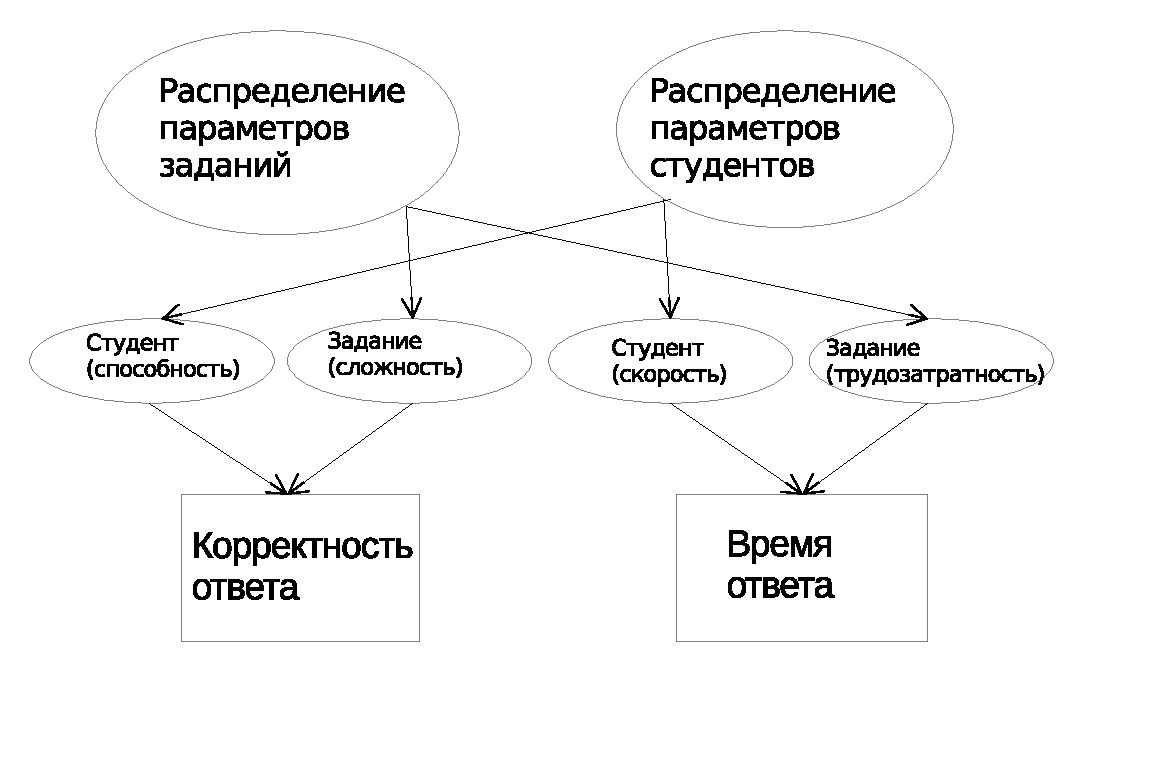
\includegraphics[scale=0.95]{VdLmodelRUS.eps}
\caption{Двухуровневая иерархическая модель}
\label{2levelfrwork}
\end{figure}

Как видно, модель имеет два уровня. На первом уровне расположены вероятностные модели для корректности ответа студента и времени ответа студента. На втором уровне вероятностная модель распределения параметров  моделей первого уровня - способность студента и его скорость для студентов всех групп и вероятностная модель распределения параметров сложности и трудозатрат для каждой задачи из пула. Рассмотрим эти модели более подробно.

В соответствии с идеями, описанными во введении к дипломной работе, время ответа и сам ответ студента (корректный или нет) являются неза\-висимыми случайными величинами. Предполагается, что параметры распре\-делений так же представляют собой реализации попарно независимых слу\-чайных величин с известными законами распределения. Исходя из сделанных предположений, запишем законы распределения параметров модели и сами модели. 

Параметры для группы студентов распределены по нормальному закону
\begin{equation}
(\theta,\tau)^T \sim N(\mu,\sigma),
\end{equation}
где $K$ - количество задач в пуле, $M$ - число студентов в группе. $(\theta,\tau)$ - двумерный вектор параметров модели, который состоит и способностей сту\-дентов и времени, с которым студенты отвечают на задания. Вектор имеет $2$-мерное нормальное распределение с вектором матема\-тического ожидания $\mu = (\mu_\theta, \mu_\tau)^T$ и ковариационной матрицей $\sigma$ размер\-ности $2\times 2$, которая в силу независимости способностей студента и времени ответа имеет блочно-диагональную структуру:
$$
\sigma = 
\left(
\begin{array}{cc}
\sigma_\theta & 0\\
0 &\sigma_\tau
\end{array}
\right)_{2\times2}
$$.

Для задачи под номером $i=1,\ldots,K$ из общего пула задач размеров $K$ ведём случайный вектор $\xi_i$ такой, что $\xi_i = (a_i,b_i,c_i,\alpha_i, \beta_i)$ - параметры задачи. Тогда $\forall i$ распределение вектора $\xi$ подчиняется $(5)$-тимерному нор\-мальному  закону:
\begin{equation}
\xi \sim N(\mu_\xi ,\Sigma_\xi ), i=1,\ldots,K
\end{equation}
где $\mu_\xi =(\mu_a,\mu_b,\mu_c,\mu_\alpha, \mu_\beta)^T$ - вектор математического ожидания и $\Sigma_\xi$ - кова\-риационная матрица для вектора  $\xi$. Независимость при распределении па\-раметров задачи не предполагается.

Для модели кор\-ректности ответа используется трёхпараметрическая ло\-гистическая модель
\begin{equation}
p_i(\theta_j) = c_i - (1-c_i)\psi[a_i(\theta_j - b_i)]; i=1,\ldots,K; j=1,\ldots,M
\end{equation}
где $\psi( * )$ - логистическая функция. Логистическая функция имеет вид
$$
\psi(z) = \frac{1}{1+e^{-z}}
$$

Время ответа студента имеет логнормальное распределение:
\label{mvonu}
\begin{equation}
\label{mainmodel}
\ln T_{ij} = \mu + \beta_i + \tau_j + \varepsilon_{ij},\quad \varepsilon_{ij} \sim N(0,\sigma^{2}_{ij}); i=1,\ldots,K; j=1,\ldots,M.
\end{equation}

Соответственно, плотность распределения времени ответа имеет следу\-ющий вид:
\begin{equation}
f(t_{ij};\tau_j,\alpha_{ij},\beta_i) = \frac{\alpha_{ij}}{\sqrt{2\pi}}exp\left\{ -\frac{1}{2}[\alpha_{ij}(\ln t_{ij} - \{\mu + \beta_i + \tau_j\})]^2 \right\},
\end{equation}
где $\alpha_{ij} = \sigma_{ij}^{-1}$.

В модели используются следующие обозначения:
$$
\begin{array}{lll}
\beta_i &-& \mbox{временной параметр, индивидуальный для задачи i}\\
\tau_j &-& \mbox{временной параметр, индивидуальный для студента j }  \\
\varepsilon_{ij} &-& \mbox{случайное отклонение}\\
\mu &-& \mbox{параметр времени, общий для всего пула задач и всех обучающихся}
\end{array}
$$

Двухуровненевая иерархическая модель, предложенная ван дер Линденом, является обобщением и расширением для двух более ранних моделей: модели Раша \cite{22.} для вероятности правильного ответа пользователя и логнормальной модели времени ответа, которую предложил Тиссен \cite{21.}. Модель ван дер Линдена позволяет ответить на ряд вопросов, которые не затрагиваются  в данной работе: например, наличие корреляции (как между параметрами задачи, так и между студентами в группе). Адаптация системы дистанционного обучения с использованием времени ответа обучающегося проходит  в рамках модели (\ref{mainmodel}). На основе описанной вероятностной модели решаются задачи выявления случаев <<нечестного>> прохождения теста и конструирования инди\-видуального варианта заданной сложности в условиях ограниченного по вре\-мени теста.

\subsubsection{Оценка параметров модели}
\label{oppmpv}

Пусть в сиcтеме дистанцинного обучения для формирования вариантов теста используется пул из $K$ задач. При этом в тестировании принимают участие $M$ студентов. Для каждого обучающегося $j$ из общего числа студентов система дистанционного обучения формирует вариант из $k$ задач. Обозначим время ответа студента $j$ на задачу $i$ как $t_{ij}$. Тогда для случайных параметров модели (\ref{mainmodel}) можно по\-лучить следующие  оценки (см. \cite{2.,6.}):
\begin{equation}
\label{1166}
\hat{\mu} = \frac{\sum\limits_{j=1}^{M}\sum\limits_{i=1}^{k}\ln t_{ij}}{k \cdot M},
\end{equation}
\begin{equation}
\hat{\beta}_i = \frac{\sum\limits_{j=1}^{M}\ln t_{ij}}{M} - \hat{\mu},
\end{equation}
\begin{equation}
\hat{\tau}_j = \frac{\sum\limits_{i=1}^{k}\ln t_{ij}}{k} - \hat{\mu},
\end{equation}
Эти оценки обладают рядом полезных свойств. Например, оценка $\hat{\tau}_j$ имеет математическое ожидание
\begin{equation}
\label{exp}
E[\hat{\tau}_j] = \tau_j
\end{equation}
и дисперсию
\begin{equation}
\label{var}
Var(\hat{\tau}_j) = \frac{\sigma^2}{k},
\end{equation}
т.е. является несмещённой и состоятельной. Наконец, оценка для дисперсии случайного отклонения $\varepsilon_{ij}$ имеет вид
\begin{equation}
\label{1167}
\hat{\sigma}^{2}_{ij} = \frac{\sum\limits_{j=1}^{M}\sum\limits_{i=1}^{k}(\ln t_{ij} - \hat{\tau}_j - \hat{\beta}_i)^2}{k \cdot M},
\end{equation}

Кроме аналитических оценок разработаны так же методы численного оце\-нивания параметров модели, например с помощью генератора Гиббса\cite{3.}, описание которых не входит в дипломную работу.

%\subsubsection{Прогнозирование времени ответа пользователя}
%\label{PVOP}
%
%Для прогнозирования времени ответа в модели используется подход, опи\-санный ниже.
%
%
%Обозначим прогнозное время ответа как $\tilde{T}_{ij}$. Тогда с учётом формул (\ref{exp}),\\(\ref{var}) получаем
%\begin{equation}
%\hat{\tau}_j \sim N\left(\tau_j, \frac{\sigma^2}{k-1}\right)
%\end{equation}
%т.к.
%\begin{equation}
%cov(\hat{\tau}_j,\varepsilon_{ij}) = 0,
%\end{equation}
%то получаем прогнозное время ответа студента на задачу \cite{5.}:
%\begin{equation}
%\label{predictedtime}
%\ln \tilde{T}_{ij} \sim N\left(\mu + \beta_i + \tau_j,\frac{k\sigma^2}{k-1}\right)
%\end{equation}

%Таким образом, прогнозное время ответа студента на задачу имеет гаус\-совское распределение.
